%%%%%%%%%%%%%%%%%%%%%%%%%%%%%%%%%%%%%%%%%%%%%%%%%%%%%%%%%%%%%
%% HEADER
%%%%%%%%%%%%%%%%%%%%%%%%%%%%%%%%%%%%%%%%%%%%%%%%%%%%%%%%%%%%%

\documentclass[a4paper, twocolumn, oneside, 10pt]{article}

\usepackage{fourier}
\usepackage[T1]{fontenc}

\usepackage{amssymb}
\usepackage{graphicx}
\usepackage{rotating}
\usepackage{pdflscape} 
\usepackage{abstract}
\usepackage[ table ]{ xcolor }
\usepackage[square, comma, sort&compress, longnamesfirst]{natbib} %
\usepackage{subfigure}
\usepackage{setspace}
%\singlespacing %% 1-spacing (default)s
%\onehalfspacing
\newcommand{\degree}{$^{\circ}$\ }
%%% END Article customizations

%%% The "real" document content comes below...


\title{The saccadic flow baseline: Accounting for image-independent biases in fixation behaviour }

\author{Alasdair D. F. Clarke, Matthew J. Stainer, Ben Tatler \& Amelia R. Hunt}

\begin{document}

\twocolumn[
\maketitle
\begin{onecolabstract}
Much effort has been made to explain eye guidance during natural scene viewing. However, a substantial component of fixation placement appears to be a set of consistent biases in eye movement behaviour. We introduce the concept of \textit{saccadic flow}, a generalisation of the central bias that describes the image-independent conditional probability of making a saccade to $(x_{i+1},y_{i+1})$, given a fixation at $(x_i,y_i)$. We suggest that saccadic flow can be used as a useful prior when carrying out analysis into fixation locations, and can be used as a sub-module in models of eye movements during scene viewing. We demonstrate the utility of this idea by presenting bias-weighted gaze landscapes, and show that there is a link between the likelihood of a saccade under the flow model, and the salience of the following fixation. We also present a minor improvement to the central bias (based on using a multivariate truncated Gaussian), and investigate the leftwards and coarse-to-fine biases. 
\end{onecolabstract}
]

%%%%%%%%%%%%%%%%%%%%%%%%%%%%%%%%%%%%%%%%%%%%%%%%%%%%%%%%%%
\section{Introduction}
%%%%%%%%%%%%%%%%%%%%%%%%%%%%%%%%%%%%%%%%%%%%%%%%%%%%%%%%%%

The human fovea provides a small window of high acuity vision to the world, and the locations that we select to view through this window can tell us how we seek the information necessary to complete the task we are currently undertaking. Fixation locations are selected based on a combination of low-level factors such as visual salience \citep{borji2013} and high-level factors \citep{yarbus1967, buswell1935, land2001}. However, there are also strong observable biases in eye movements that are independent of the content of the scene or the task being performed \citep{tatler-vincent2009, foulsham2010}, such as a strong tendency to fixate near to the centre of images \citep{tatler2007, canosa2003, stainer2013}. If we are to gain a complete understanding of the factors that govern how we sample information, we must build models of eye guidance on the framework of these underlying biases, using them as a baseline against which to compare effects of the scene, task, image properties and individual differences.

%%%%%%%%%%%%%%%%%%%%%%%%%%%%%%%%%%%%%%%%%%%%%%%%%%%%%%%%%%%%%
\subsection{Eye movement heuristics}
%%%%%%%%%%%%%%%%%%%%%%%%%%%%%%%%%%%%%%%%%%%%%%%%%%%%%%%%%%%%%

One of the most influential models of eye movements of the last decade is the optimal search model \citep{najemnik-geisler2008}, which posits that human saccadic behaviour during visual search is consistent with predictions made by an ideal observer. The number of fixations human observers needed to make to find the target was closely matched by the ideal observer model, in which successive fixations were selected based on reducing uncertainty about the target's location, taking into account search history and target visibility across the visual field. The efficiency of human search (at least, in search for a Gabor patch hidden in $1/f$-noise) suggests this as a plausible mechanism for selecting fixations during search. Further evidence for this theory comes from \cite{ma2011} who find that human observers are near-optimal in a visual search task with line segments, and presented a neural network implementation of near-optimal search based on probabilistic population coding.  

While this modelling framework is attractive, there are several issues. The computations driving each fixation are complex, and depend on a fairly precise representation of one's own acuity over the visual field for a wide range of possible target/background combinations. One might therefore question the assumption that these computations are undertaken to determine the location of each of the 3-4 fixations made on average every second during visual search. More importantly,  \cite{morvan-maloney2012} demonstrated that human observers are not able to use information about visual sensitivity in the periphery to rationally plan even a a single saccade to the optimal location in a target discrimination task. In their experiment, the observer simply has to select a location from which to detect a target that can appear with equal probability in one of two possible locations. If the locations are relatively close together, a location in between will maximise the probability of detecting a target appearing in either location. When the targets are too far apart to reliably detect the target from a point equidistant between them, the rational strategy is to look directly at one of the two possible target locations. Inconsistent with optimal viewing strategies, however, the observers did not systematically modify their choice about where to fixate according to the distance between the possible target locations. This striking failure of optimality has recently been replicated in a larger sample and generalised to other decisions in addition to eye movements  \citep{clarke-hunt2015}. To reconcile their results with those of  \cite{najemnik-geisler2008},  \cite{morvan-maloney2012} suggest \textit{heuristics} guide saccade planning; that is, basic oculomotor biases such as a tendency to make saccades of particular amplitudes, and/or to particular regions of a display, or in particular sequences, depending on the current task. 

This idea has recently been formalised in a model by \cite{clarke2015}, who demonstrate that a stochastic search model based on a memoryless random walk can find a target in noise in a similar number of fixations to human observers. The key component of this model was the use of the empirical distribution of saccades: for each saccade the model randomly samples a saccade from distributions estimating the likelihood a human observer made a saccade from $(x_{i+1},y_{i+1})$ to $(x_i,y_i)$. This stochastic model differs from the random baseline implemented by \cite{najemnik-geisler2008}, in which they randomly selected each fixation location from all possible points in the display, because it incorporates basic oculomotor heuristics that guide the eyes, without the need for complex computation of peripheral sensitivity or target location probability. In this paper, we re-implement and generalise this model, named \textit{saccadic flow}, and examine the extent to which it is useful as a prior for analysing eye movements made with more natural (photographic) stimuli. This concept is illustrated in Figure \ref{fig:empiricalSaccadicFlow}. 
\begin{figure}[htb]
\centering
\subfigure{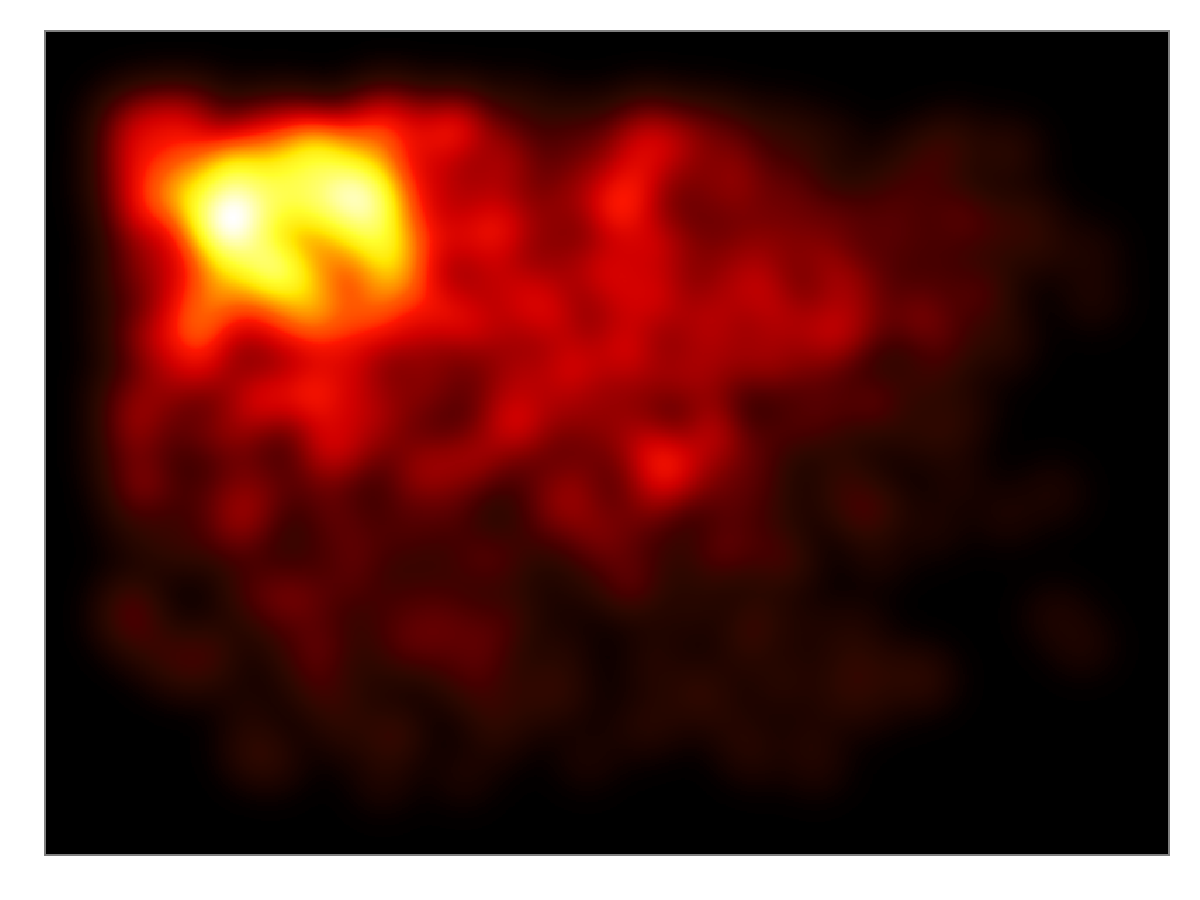
\includegraphics[width=2.5cm]{../scripts/heatmaps/SaccadicFlowMaps/Figures/BBias_11.pdf}}
\subfigure{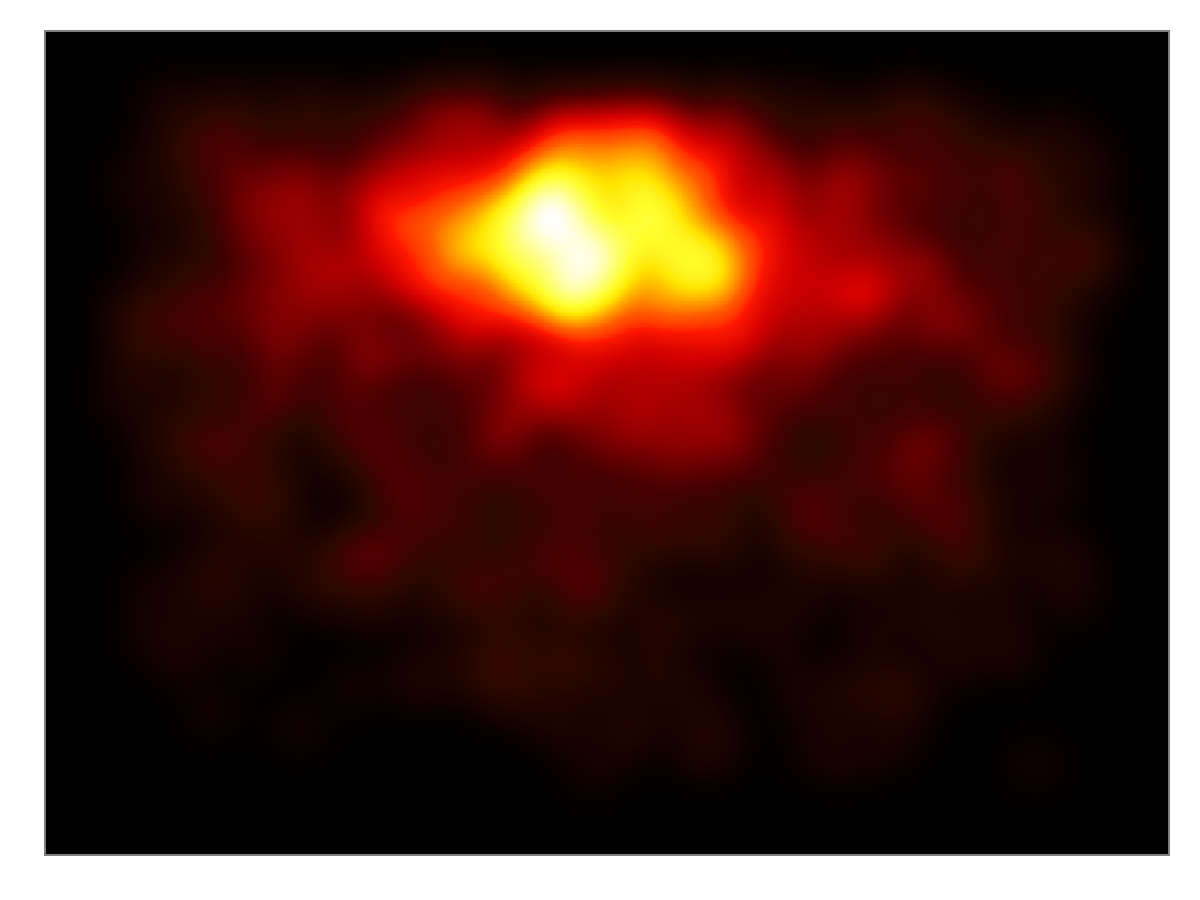
\includegraphics[width=2.5cm]{../scripts/heatmaps/SaccadicFlowMaps/Figures/BBias_12.pdf}}
\subfigure{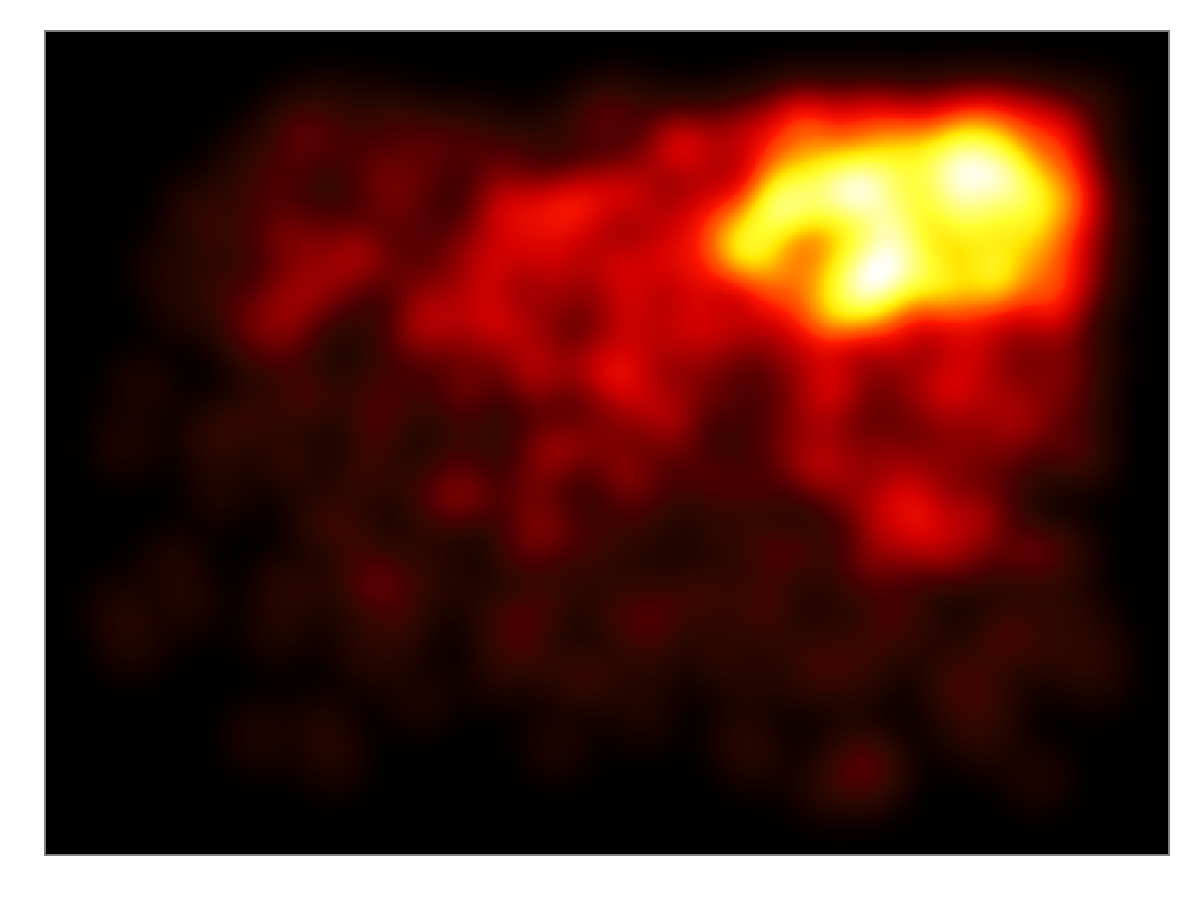
\includegraphics[width=2.5cm]{../scripts/heatmaps/SaccadicFlowMaps/Figures/BBias_13.pdf}}
\subfigure{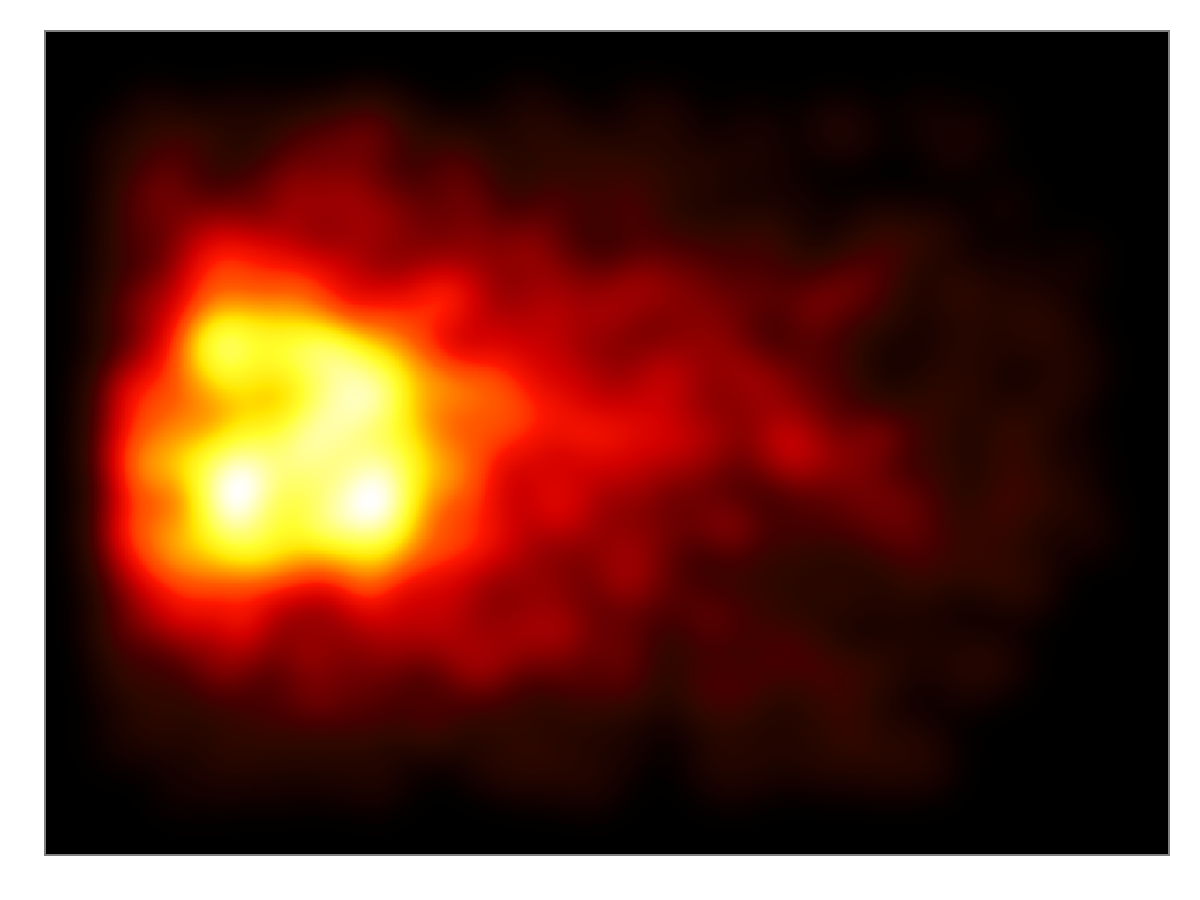
\includegraphics[width=2.5cm]{../scripts/heatmaps/SaccadicFlowMaps/Figures/BBias_21.pdf}}
\subfigure{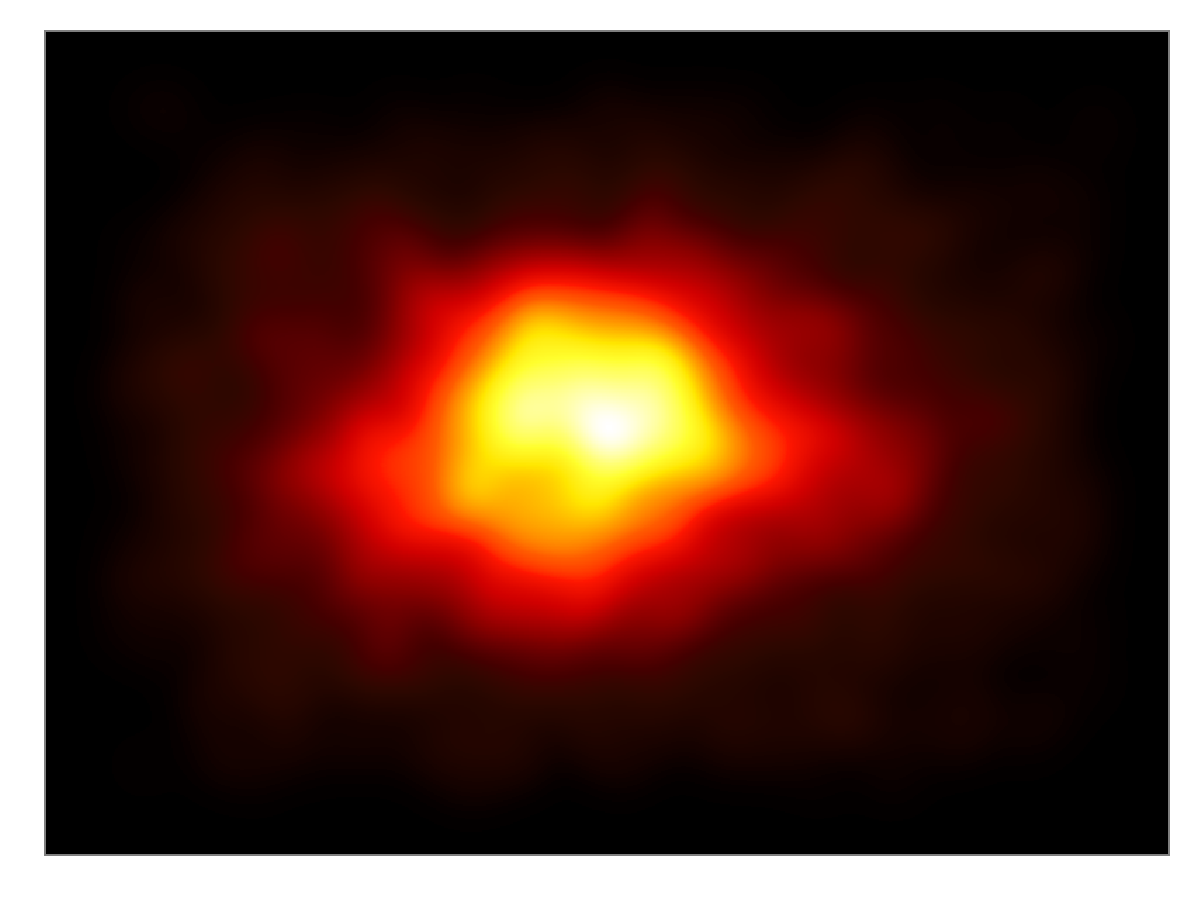
\includegraphics[width=2.5cm]{../scripts/heatmaps/SaccadicFlowMaps/Figures/BBias_22.pdf}}
\subfigure{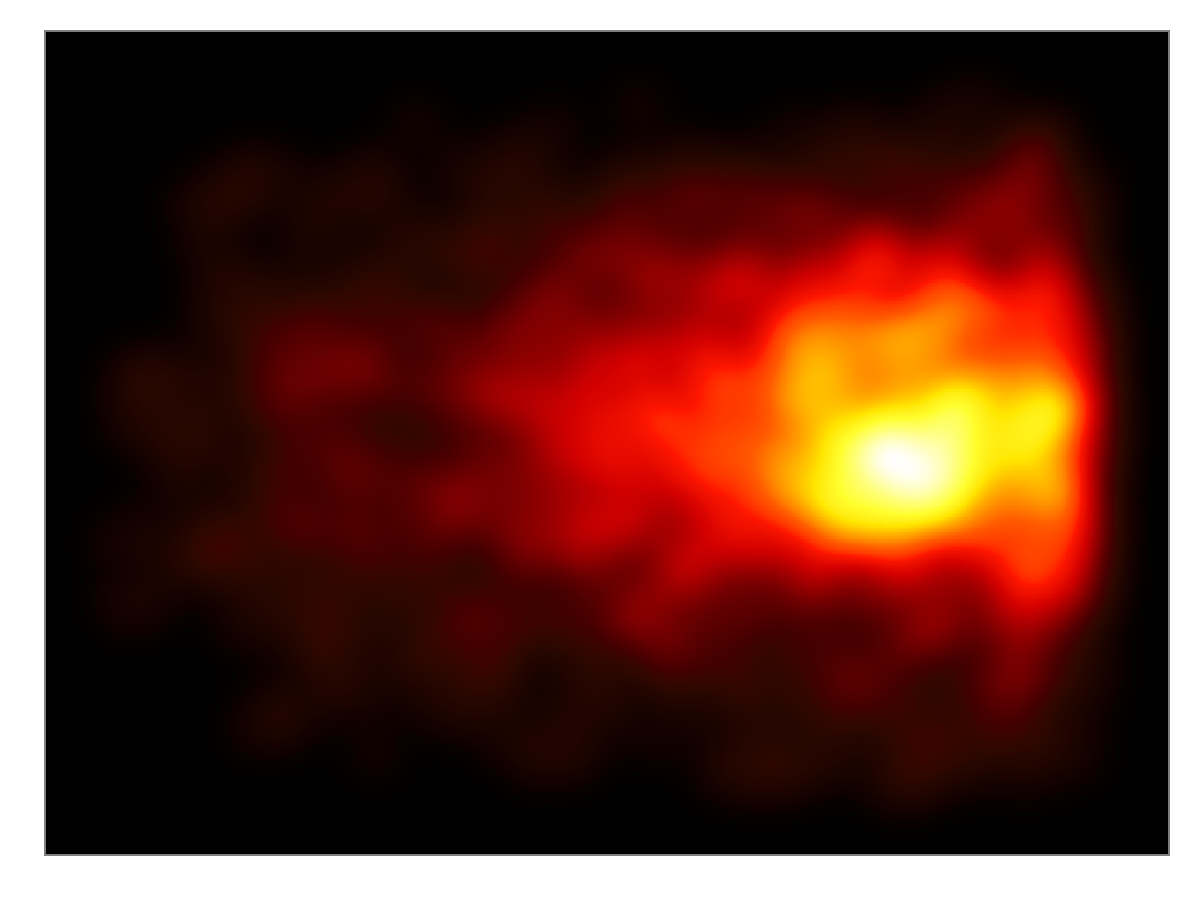
\includegraphics[width=2.5cm]{../scripts/heatmaps/SaccadicFlowMaps/Figures/BBias_23.pdf}}
\subfigure{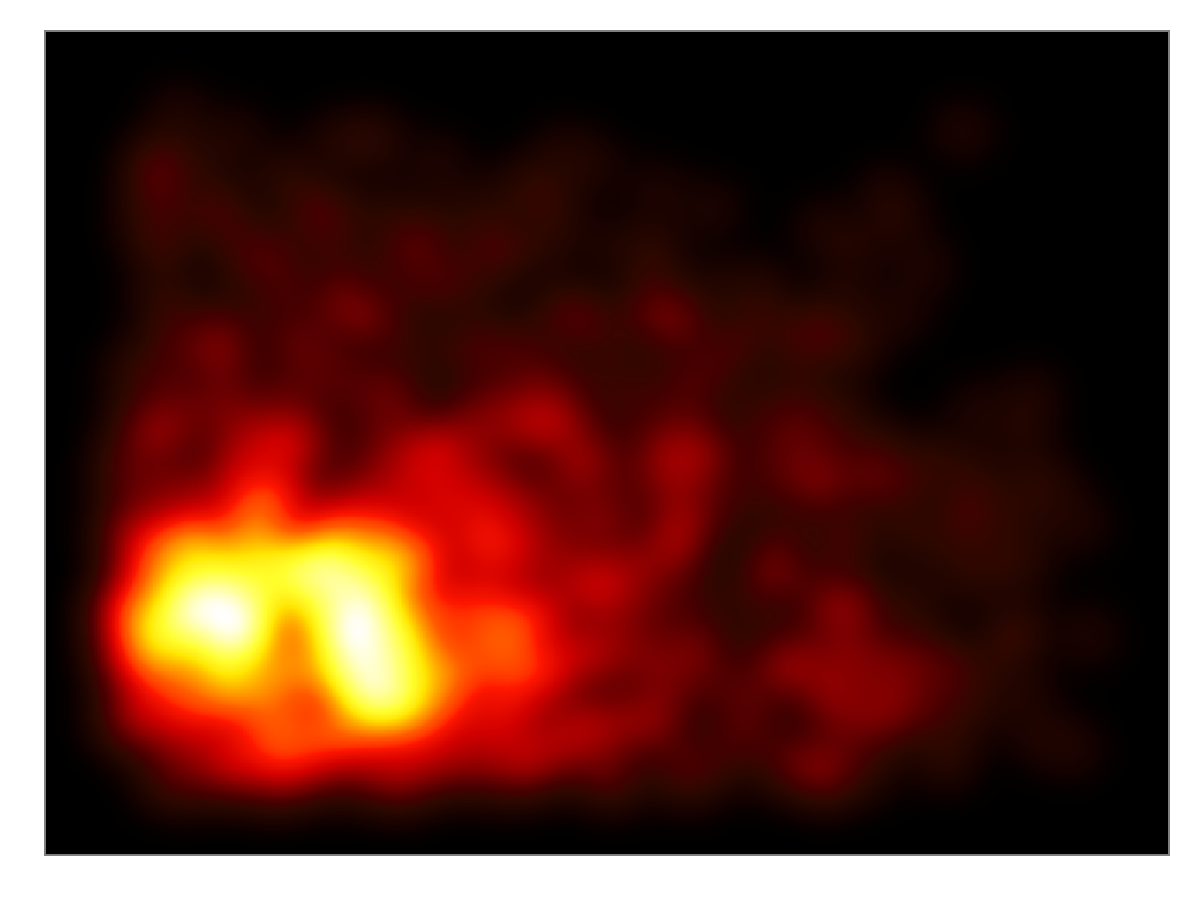
\includegraphics[width=2.5cm]{../scripts/heatmaps/SaccadicFlowMaps/Figures/BBias_31.pdf}}
\subfigure{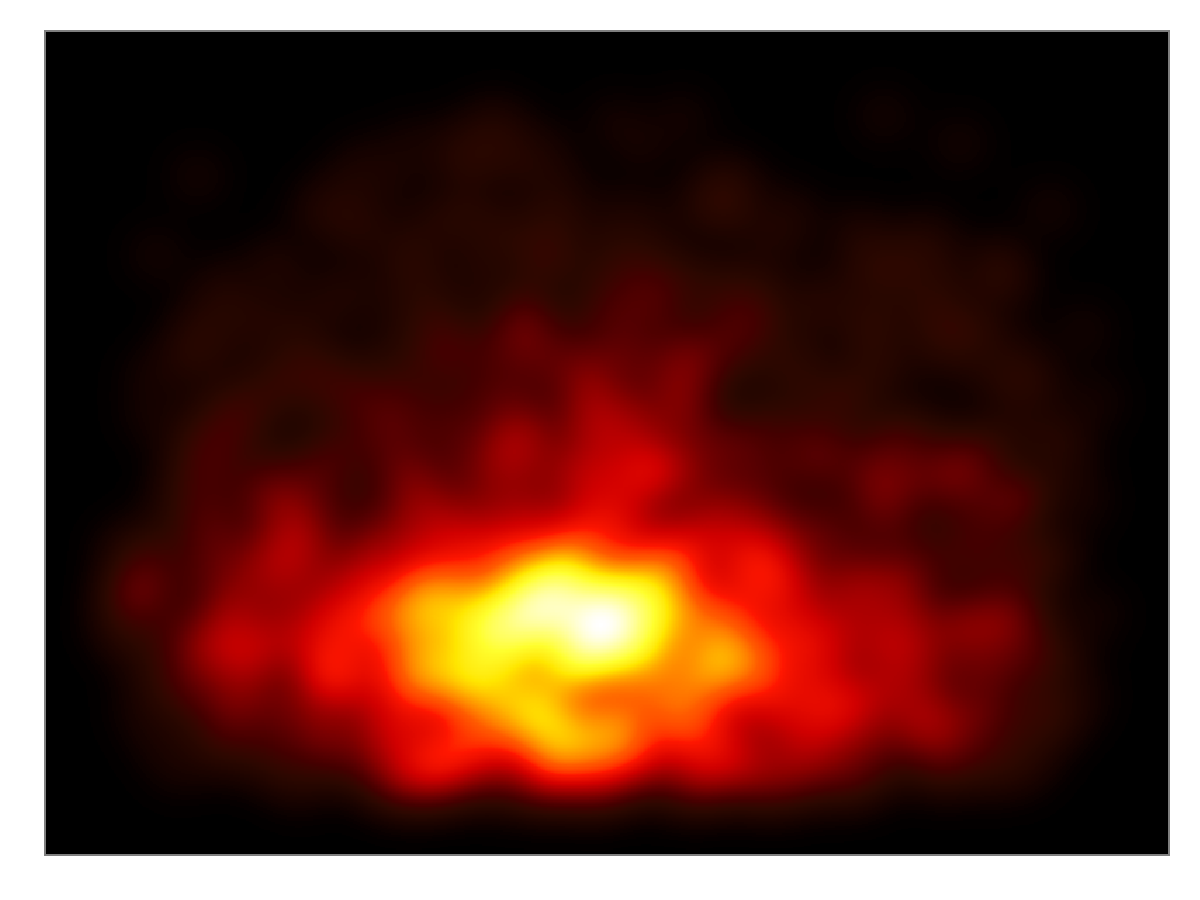
\includegraphics[width=2.5cm]{../scripts/heatmaps/SaccadicFlowMaps/Figures/BBias_32.pdf}}
\subfigure{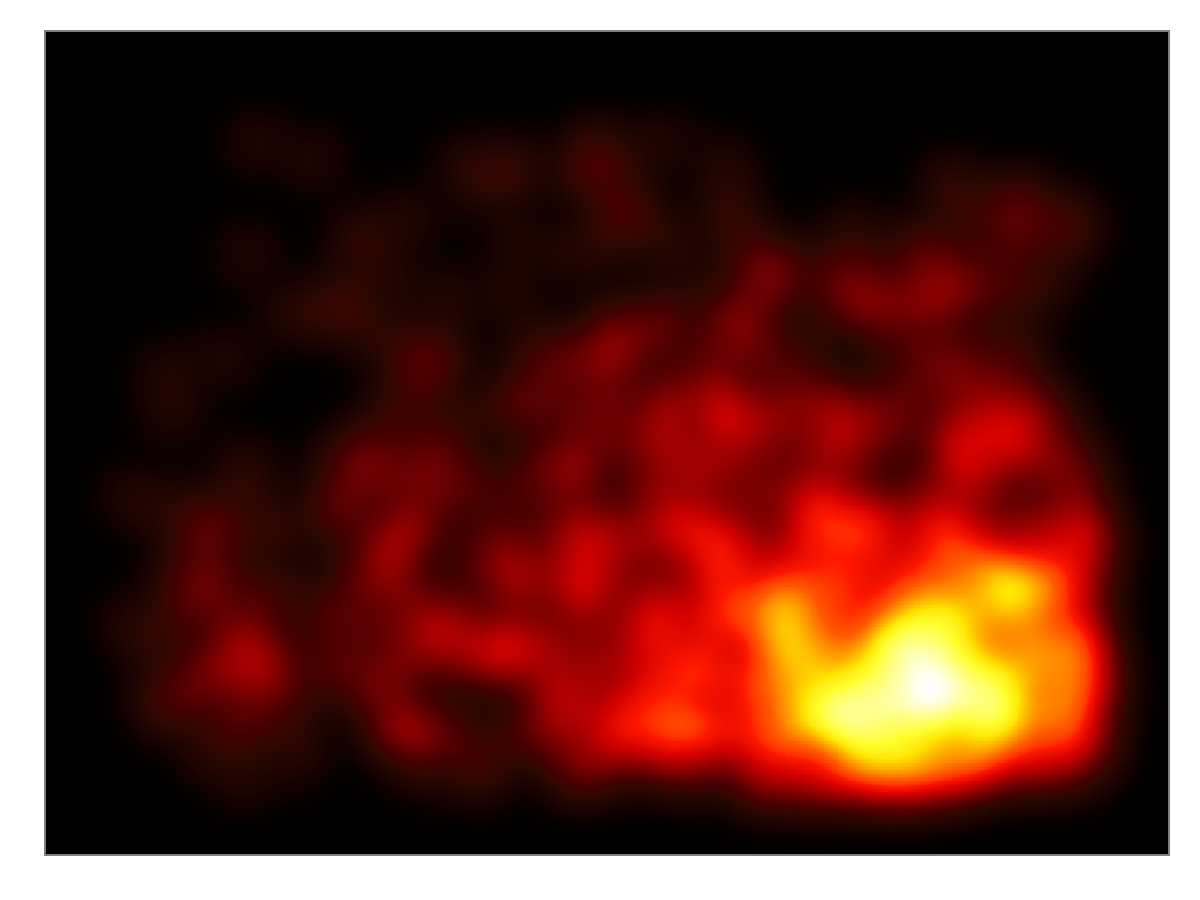
\includegraphics[width=2.5cm]{../scripts/heatmaps/SaccadicFlowMaps/Figures/BBias_33.pdf}}
\caption{Saccade landing positions from fixations that were in different sections of the screen. Data from each plot has been separated into fixations in 9 spatial bins, with the screen being divided into thirds in both horizontal and vertical aspects.}
\label{fig:empiricalSaccadicFlow}
\end{figure}

%%%%%%%%%%%%%%%%%%%%%%%%%%%%%%%%%%%%%%%%%%%%%%%%%%%%%%%%%%%%%
\subsection{The central bias}
%%%%%%%%%%%%%%%%%%%%%%%%%%%%%%%%%%%%%%%%%%%%%%%%%%%%%%%%%%%%%
 
There is a strong tendency for people to look close to the centre of pictures \citep{tatler2007, tatler2005, canosa2003, clarke-tatler2014} and videos \citep{tseng2009,loschky2015} presented on computer screens. There have been a number of suggestions for why this might be, the simplest being that the centre of the stimuli is the best place to look in terms of making best use of parafoveal vision. One possibility for this effect is that the muscles of the eye show a preference for the `straight ahead' position, re-centring in the orbit of the eye socket for most comfortable contraction of the ocular muscles (an \emph{orbital reserve} \citep{fuller1996}). As most scene viewing experimental set-ups stabilise the head to increase the accuracy of the eye tracking, and most scenes are presented in the centre of computer displays, such a re-centring mechanism would mean that the centre of images would indeed be preferentially selected. However, when scenes are scrambled into four quadrants, fixations are located near to the centre of each quadrant, rather than the display centre, suggesting that the central tendency is responsive to the viewed content \citep{stainer2013} rather than the frames of the computer monitor.

Another possibility for the central fixation bias is that it represents a \emph{photographer bias} as photographers tend to frame their shots to include the most important content in the centre of the scene. However, when \cite{tatler2007} presented scenes where the image features were biased towards the edge of the scene, the central fixation bias persisted. The final possibility is that as a consequence of repeated exposure to photographer bias, the centre of scenes is simply where people are \emph{trained} to look at images \citep{parkhurst2002}. Such learning of spatial probabilities of targets can explain why, for example, people tend to look around the horizon when searching for people in natural scenes \citep{birmingham2009, torralba2006, ehinger2009}. Expecting to find interesting content in the centre of scenes might be a consequence of this hypothesis typically being correct. 

\cite{clarke-tatler2014} revealed that the characteristics of the central bias are remarkably consistent across a series of eye movement databases over tasks such as free-viewing, visual search and object naming. They proposed a simple, standardised central baseline based on a multivariate Gaussian, an demonstrated that it outperforms similar measures previously used in the literature.

\subsection{Other Behavioural biases in saccades}
While the central bias has attracted the most attention (at least in terms of models of visual attention), a number of other biases have been documented. These are discussed below. 

\textit{Horizontal Saccades}: Several researchers have noted that when viewing scenes there is a higher proportion of eye movements in horizontal directions than vertical or oblique movements \citep[e.g.][]{gilchrist2006,foulsham2008,tatler-vincent2009,lappe1998,lee2002}. There are a number of possibilities as to why this tendency exists. Firstly, there may be a muscular or neural dominance making oculomotor movements in the horizontal directions more likely. Secondly, the characteristics of photographic images may mean that content tends to be arranged horizontally by the photographer. In such situations, horizontal saccades may be the most efficient way to inspect scenes. Thirdly, using horizontal saccades in scene viewing might be a learned strategy. Observers may learn the natural characteristics of scenes based on previous experience, and therefore demonstrate an increased likelihood of moving in the horizontal direction. A final alternative explanation is that this tendency is a consequence of the aspect ratio of visual displays, which normally allow for larger amplitude saccades in the horizontal than vertical directions \citep{wartburg2007}.

Results from Foulsham and colleagues suggest that the photographer bias explanation may be the most important. \cite{foulsham2008} found that when the orientation of an image is rotated, the distribution of saccade directions follows the orientation of the scene. A second exception comes from using circular apertures \citep{foulsham-kingstone2010}. When a scene is presented in a circular aperture, the tendency to make horizontal saccades disappears, being replaced by a tendency to make vertical saccades relative to the image orientation. However, when using fractal images (where images do not have an obvious orientation), observers tend make horizontal saccades, regardless of the angle that the image is presented.

\textit{Coarse-to-fine}: Another robust pattern in human saccadic behaviour is the tendency to make large eye movements after the initial scene onset, and smaller saccades as the trial unfolds \citep{over2007, pannasch2008,antes1974}. This is often accompanied by an increase in fixation durations,  and is framed as a move from ambient to focal processing \citep{follet2011}. \cite{godwin2014} successfully replicated these findings, but they offered an alternative explanation, namely that this behaviours is driven stochastic factors that govern eye movements.


\textit{Leftwards bias}: Several studies have shown that observers exhibit a bias to fixate the left half of a stimulus over the right \citep{ossandon2014,nuthmann-matthias2014,learmonth2015,zelinsky1996, brandt1945}. This effects falls under the more general spatial attention bias of psuedoneglect \citep{bowers-heilman1980}, which also effects tasks such as line bisection tasks. The leftwards bias is typically short-lived, effecting only the first couple of saccades after scene onset, and while it is robust, it is comparatively weak compared to other biases in scene viewing. For example,  \cite{dickinson-intraub2009} found $62\%$ of initial saccades were directed to the left half of the image during free viewing. There is some evidence that this bias is related to native reading direction \citep{friedrich2014}.

\textit{Saccadic Momentum and Inhibition of Return}: Several studies have described sequential dependencies during free viewing that bias saccades to repeat the same vector and amplitude (known as saccadic momentum) and to bias saccades away from returning to previously-visited targets (known as inhibition of return). Although both of these phenomena bias fixations away from previously-fixated locations, they differ in that inhibition of return is bound to a location in the search array, i.e. it is coded in object-based or spatiotopic coordinates (e.g. \cite{krueger-hunt2013}), while saccadic momentum has been characterised as a basic tendency to repeat the same motor program \citep{wang2011}. Inhibition of return, unlike saccadic momentum, is task-dependent \citep{dodd2009} and is disrupted by removing the scene or inhibited object  \citep{klein-macinnes1999, takeda-yagi2000}.  \cite{macinnes2014} observed both of these mechanisms operating during free visual search of a complex scene, but presumably only saccadic momentum would be consistently observed for all tasks and images. 

\subsection{The present study}

These biases, in particular, the central bias, are important to take into account when evaluating the performance of models of fixation location, and investigating relationships between eye movement data and other factors. The main contribution of this manuscript is to introduce the \textit{saccadic flow} model. This can be thought of as a generalisation of the central bias: instead of simply characterising the image-independent probability of fixating $(x_i, y_i)$ we model the conditional probabilities $p(x_i,y_i|x_{i-1}, y_{i-1})$. i.e. the probability of making a saccade from to $(x_i,y_i)$ given we are currently fixating $(x_{i-1}, y_{i-1})$.

In Section \ref{sec:usingbiases} we demonstrate how the central bias and saccadic flow can be used as priors and components of models to improve analysis and visualisation methods. In particular, we will present bias-weighted gaze landscapes, and demonstrate an interaction between the likelihood of a saccade under different bias models and bottom-up visual salience. Finally, we will investigate the short-comings of these generative models by comparing synthesised data to human eye movements. In Section \ref{sec:biases} we will give full details of the saccadic flow model and an improved version of the central bias model. 

%%%%%%%%%%%%%%%%%%%%%%%%%%%%%%%%%%%%%%%%%%%%%%%%%%%%%%%%%%
\section{Using Biases}
\label{sec:usingbiases}
%%%%%%%%%%%%%%%%%%%%%%%%%%%%%%%%%%%%%%%%%%%%%%%%%%%%%%%%%%

This section make use of an improved central bias model the \textit{saccadic flow} model (described in Section \ref{ModellingFlow}). The new central bias model is similar to the model presented by \cite{clarke-tatler2014} except for using a truncated Gaussian distribution to take the image boundaries into account. We present three examples of how these bias models can be used as a prior in order to weight fixations. First of all, we will demonstrate how we can weight fixations in gaze landscapes (also known as hotspot maps) to reduce noise and to give an improved visualisation of the image regions participants looked at more than expected. Secondly, we examine whether saccadic flow can be used to better understand the contribution of low-level features on fixation selection, and potentially lead to better evaluation of such computational saliency models. Finally, we use flow to generate a series of saccades and compare these to observed human saccades. Being able to generate realistic synthetic datasets is useful to create an image-independent baseline with which to examine spatial maps of prediction using signal detection theory \citep[see][]{clarke-tatler2014}.


\subsection{Gaze landscapes}

One technique that is commonly used to visualise the spatial allocation of gaze is to create 'heatmap' plots where colour or luminance are used to indicate the density of fixation on those locations (Figure ~\ref{fig:adjustedHeatmaps}, column 2). A potential problem with visualising data in this way is that such maps represent all fixations as being of equal importance to the inspection. For example, a fixated location with a fixation of a second would be weighted equally with fixations that lasted half that time. If we want to make an assumption that fixation duration is intimately linked with the importance of that fixation (i.e. we will look longer at more informative information) then we can change our visualisation to weight fixations by their duration (Figure ~\ref{fig:adjustedHeatmaps}, column 3).

\begin{figure*}
\centering
\includegraphics[width=13cm]{figs/heatmap_figure.pdf}
\caption{Examples of fixation heatmap plots from \cite{clarke2013}. The same fixations are presented where the Gaussian at each fixation is weighted by the duration of the fixation, the centre bias model from \citep{clarke-tatler2014} , and the saccadic flow model presented in this paper.}
\label{fig:adjustedHeatmaps}
\end{figure*}

An advantage of the \citet{clarke-tatler2014} model, and the saccadic flow model here is that we can represent fixations by the likelihood that they would occur based on the predictions of the models. As there is an image independent tendency to fixate in the centre of the scene (for example), then we might consider that saccades to locations less predicted by these behavioural and oculomotor biases might involve more high-level mechanisms. In Figure ~\ref{fig:adjustedHeatmaps} (column 4 and 5) we present some overlaid heatmap data from the \citet{clarke2013} dataset, where fixations are weighted by the inverse probability of them occurring based on the models of central bias and saccadic flow. These figures reveal that representing data in this manner can allow us to visualise information that was important enough to break the biases of looking at the scene centre, or making saccades in line with our saccadic flow model. We can therefore use this to provide visualisations that remove some of the image-independent biases, and reveal the more important image \emph{dependent} information.


The top row of Figure ~\ref{fig:adjustedHeatmaps} demonstrates that weighting the fixations by the central bias and flow model both reduce the \emph{importance} of some fixations. The central bias model punishes fixations near the center of the image, while the flow model punishes fixations that were well predicted by the oculomotor biases of the saccadic flow model. Conversely, the models reward unlikely fixations. The second row reveals an instance of where the car to the left received less fixations than the pub sign, but that these fixations are boosted in the central bias and saccadic flow models where 'unlikely' saccades were made to this location. In the third and fourth rows, there are examples of images with a photographer bias of content towards the centre of the photograph. This reveals an example of where down-weighting the central fixations might lose important content.
where the central bias model reduces the influence fixations in the centre of pictures that have important content located there. Given the tendency for photographers to bias their photographs in the centre, reducing fixations to the castle in the painting (row 3) and the girl's face (row 4) would perhaps punish centrally biased photographic composition. With the flow model, these areas are still represented as observers made saccades unlikely to be driven by behavioural biases to these regions.

\subsection{Removing biases when examining image-dependent information}

By considering saccades by the probability that they were generated by the non-image biases, we can gain further insights into the image-dependent features that are important in attracting fixation. One feature that has been shown to correlate with fixation is visual salience (e.g. Parkhurst?). However, others have argued that this tendency is driven by the correlation between salient objects and the central bias (XXHenderson?XX), and that the oculomotor biases which favour a central tendency would give same fixation placement regardless of saliency \citep{tatler-vincent2009}. Here, we can examine this question by looking at the relationship between saccade probability and the ability of different conspicuity maps to predict fixation. We can therefore examine how the effect of visual salience observed in eye movement analysis is related to the behavioural biases of eye movement.

We examined the proportion of fixations that fell in the brightest 20\% of pixels of salience maps by saccade likelihood from the flow and central bias models. Fixations were separated for each image into bins of 5\% from the least-likely to the most-likely to be generated based on salience. We then examined what proportion of each of these bins were in the brightest 20\% of salience maps using the Artificial Whitening Saliency (AWS; \cite{garciadiaz2012}), RARE \citep{riche2013} and Graph-based visual saliency \citep[GBVS;][]{harel2006} algorithms. We selected AWS and RARE as they are the two best performing salience models according to the MIT Saliency Benchmark \citep{mit-saliency-benchmark,judd2012} with publicly available code, and GBVS as it contains a bias towards the centre cause by summing neighbouring pixel values across the spatial prediction map.

Figure ~\ref{fig:salmaps} reveals that the probability of making a saccade based on both the central bias and the flow model is highly related to salience in AWS and RARE, with low-likelihood saccades being less likely to be to a salient region. Saccades that are very unlikely to be generated based on the oculomotor tendencies of eye movement (both flow and central bias) as therefore also less well explained by salience. This means that it may be important to consider, and potentially remove behavioural biases when attempting to predict fixation selection using feature-based models to ensure that any benefit in predictive power cannot be explained by behavioural biases correlating with, for example, central biases. When examining a model that contains an inherent central bias (GBVS), we can see that weighting fixations by the \citet{clarke-tatler2014} central bias model is highly related to the performance of GBVS in predicting fixation selection.

%Examples of the maps can be seen in Figure \ref{fig:salmaps}. Salience maps were normalised to sum to 1, and data were analysed using linear mixed-effect models with the fixation weighting (duration, central bias or saccadic flow) as fixed effect factors, and image and participant as random effects. 

\begin{figure}
\centering
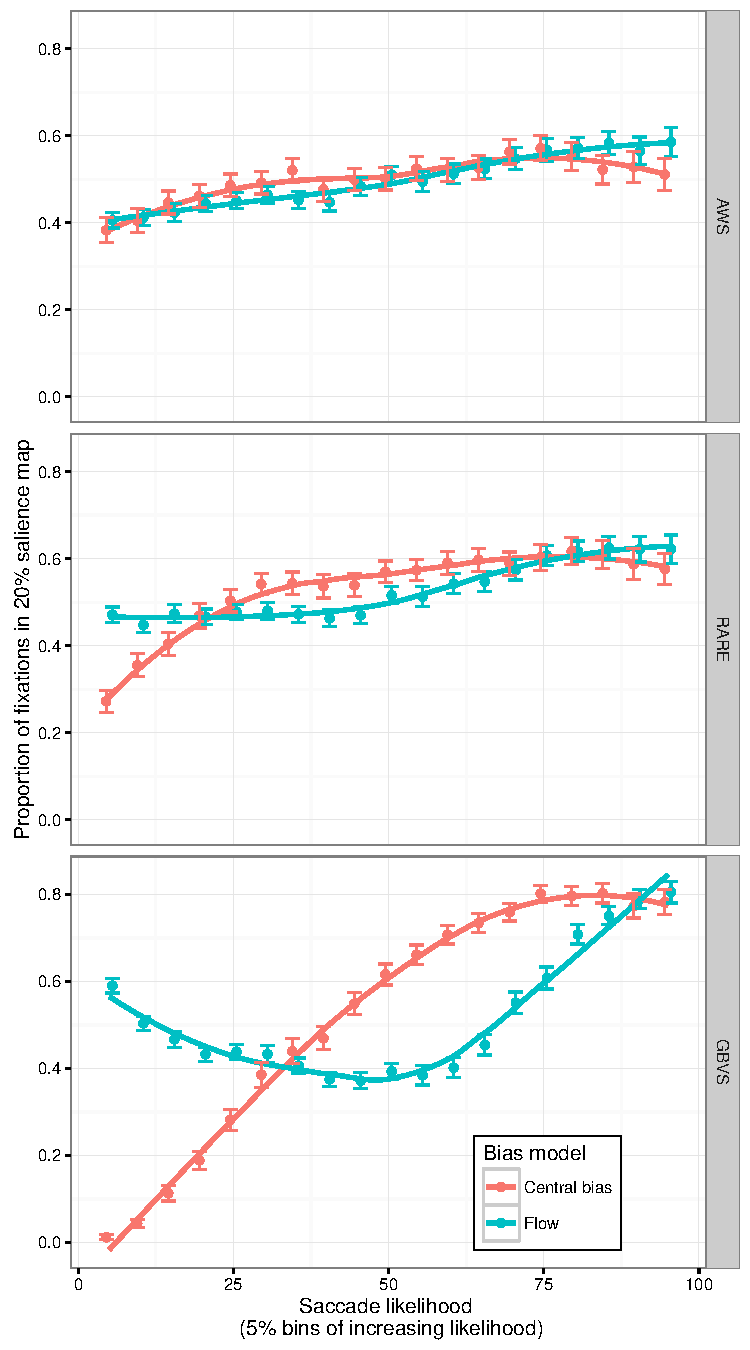
\includegraphics[width=\columnwidth]{figs/SaccadeSaliency.pdf}
\caption{Saccades binned by probability of them occurring in 5\% bins against the proportion of those fixations that fell in a 20\% thresholded region of AWS, RARE and GBVS salience maps.}
\label{fig:salmaps}
\end{figure}




% \subsubsection{Clarke 2013}

%There was no relationship between the duration of a fixation and salience using any of the three algorithms (all \emph{p}'s > .05). The relationship between the probability of saccades occurring based on the central bias model and the visual salience of the landing position did not quite reach significance using AWS (\emph{p}=.065), but was significant when using the RARE algorithm (\emph{p}<.001), with a strong positive correlation confirming that saccades that landed close to the image centre were also highly salient, whereas fixations that were further from the centre were less salient. This was supported when using a centrally-biased salience algorithm (GBVS) in which a stronger relationship was observed. Finally, saccadic flow was significantly related to salience in all models, with saccades that were unlikely to be driven by behavioural bias having much lower salience scores than saccades that could be explained by the flow model. 


%\begin{table*}
%    \centering
%    \caption{\label{tab:salienceAUC} Linear Mixed-effect model outputs for relationship between duration, central bias and saccadic flow salience at fixation in the Clarke et al., (2013) dataset.}
%    \begin{tabular}{cccccc}
%           Salience model 	& Fixation weighting 	& $\beta$ 		& SE 		& \emph{t} 	& \emph{p} \\ \hline
%           AWS	\\
%           	& Duration 				&  2.28e-09		& 2.95e-08 	& 0.08 		& .996 \\
%           					& Central bias 			&  5.5e-07 		& 2.71e-07	& 2.03		& .065 . \\
%          					& Saccadic flow 		&  1.82e-07		& 2.09e-08 	& 8.724     & <.001*** \\
%
%		   RARE \\
%		   	& Duration 				&  -1.52e-08 	& 3.82e-08 	& -0.4 		& .89 \\
%           				& Central bias 			&  1.39e-06 	& 3.95e-07 	& 3.51 		& <.001*** \\
%          				& Saccadic flow 		&  2.31e-07 	& 3.35e-08 	& 6.89 		& <.001*** \\
%
%           GBVS  \\
%           	& Duration 				&  -3.93e-09 	& 1.94e-08 	& -0.2 		& .973 \\
%           				& Central bias 			&  3.34e-06 	& 1.69e-07 	& 19.79 	& <.001*** \\
%          				& Saccadic flow 		&  1.29e-07 	& 1.83e-08 	& 7.03 		& <.001*** \\
%   \\ \hline         
%    \end{tabular}
% \end{table*}
%

\subsection{Saccadic Flow as a Generative Model}
\label{sec:humanComp}

Another use of the saccadic flow model is to generate sequences of synthetic scan-paths. We can then compare the distributions with empirical scan-paths to determine which aspects of human saccadic behaviour are not captured by our model. To do this, we will create a merged dataset of fixations from the eight training datasets (175 000 fixations, including initial fixations, in total over 16 000 trials), and then generate a matched synthetic dataset such that the number of fixations in each trial is identical. 

We can see from Figure \ref{fig:flowHumanComp}(a) and (b) that both the central bias and the saccadic flow model do an good job of capturing the distribution of fixation locations over the $x$ and $y$ axes. While it is not surprising that the central bias closely matches the empirical distributions (as this is exactly what it has been fitted to), it is interesting that saccadic flow does just as good a job. Hence, the central bias can be thought of as a property of saccadic flow, and does not need to be accounted for separately. 

When compared to the empirical distributions, both the central bias and saccadic flow appear to be slightly biased towards making fixations to the extreme edges of the image. This suggests that the truncated Gaussian distribution does not quite capture the effects of the image boundary on fixation selection and there is some additional aversion to fixating close to the screen edge. 

Another discrepancy between the synthetic and empirical distributions can be seen with saccadic amplitudes. While the flow model is a better fit to the human data than the central bias, it still underestimates the proportion of very short saccades (Figure \ref{fig:flowHumanComp}(c)). Interestingly, the flow model does manage to capture the initial increase in saccadic amplitudes after scene onset (Figure \ref{fig:flowHumanComp}(d)), but it does not explain the subsequent coarse-to-fine dynamics that are seen in the empirical scan-paths. 


\begin{figure}[htb]
\centering
\subfigure[]{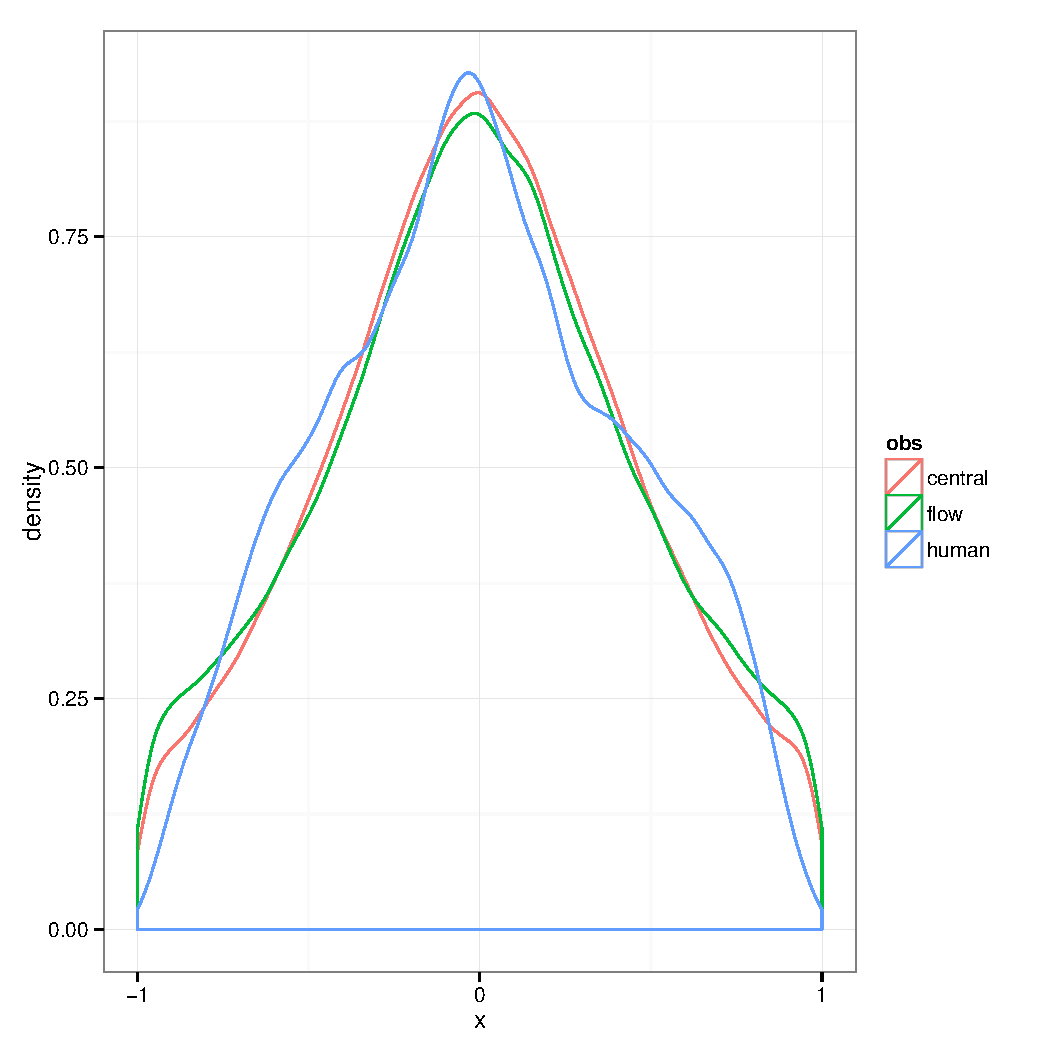
\includegraphics[width=3.8cm]{../scripts/coarse2fine/figs/xFixComparison}}
\subfigure[]{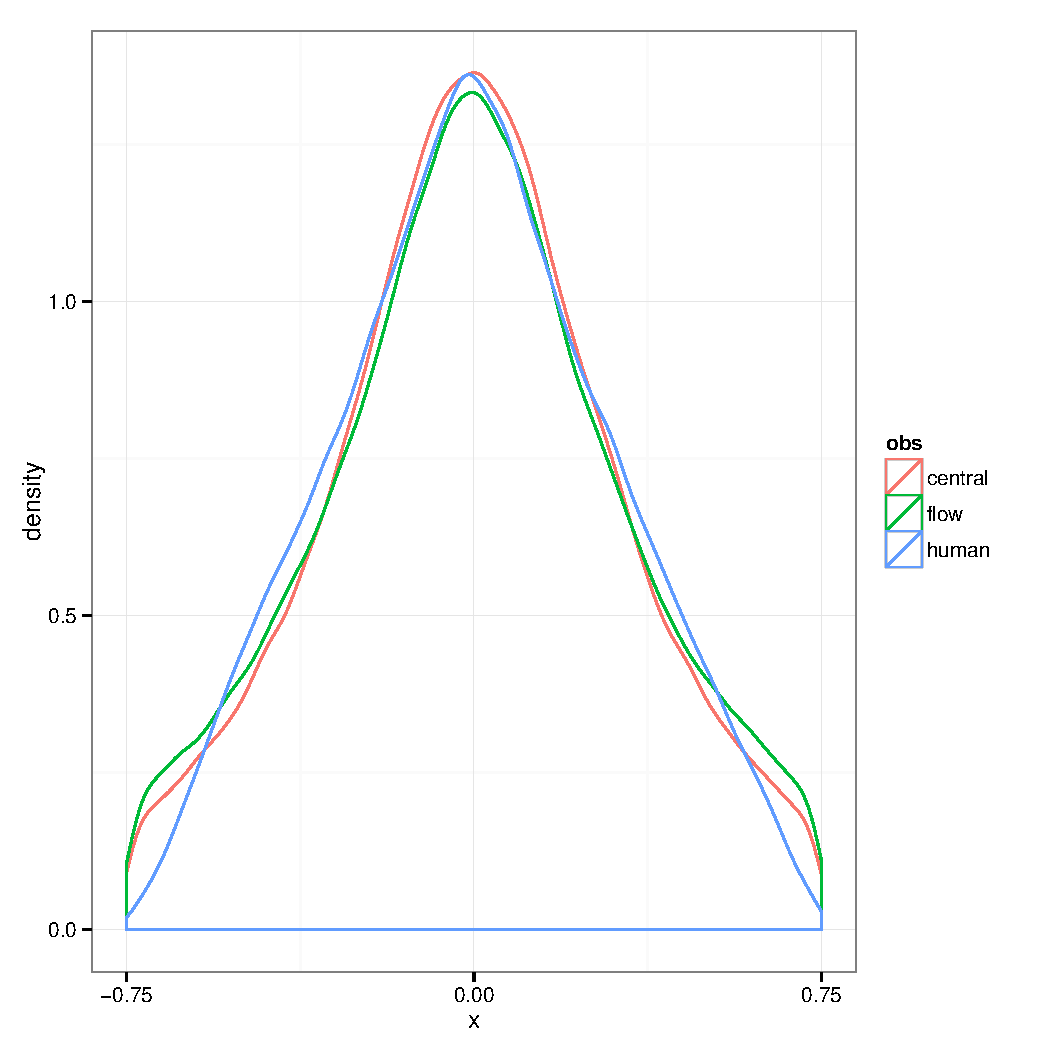
\includegraphics[width=3.8cm]{../scripts/coarse2fine/figs/yFixComparison}}
\subfigure[]{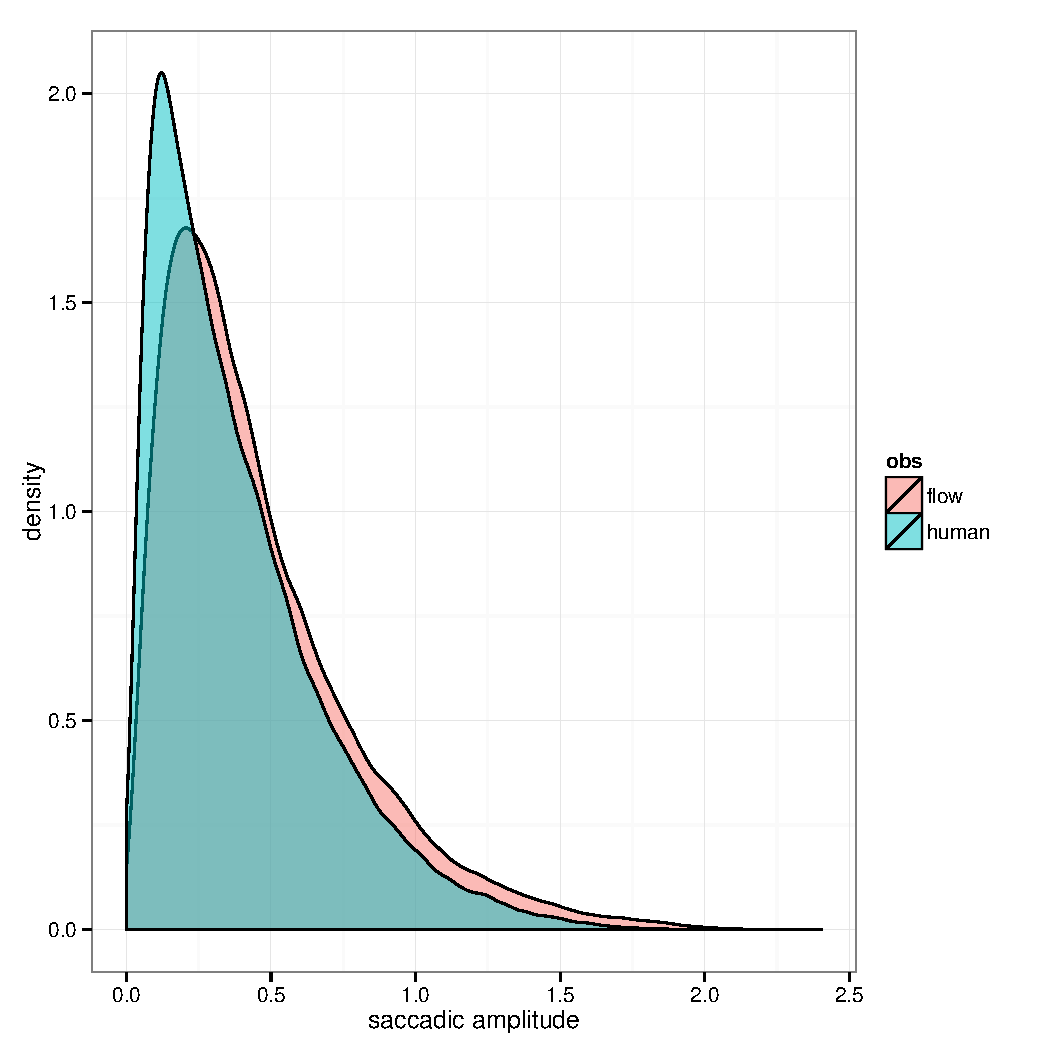
\includegraphics[width=3.8cm]{../scripts/coarse2fine/figs/ampSaccComparison}}
\subfigure[]{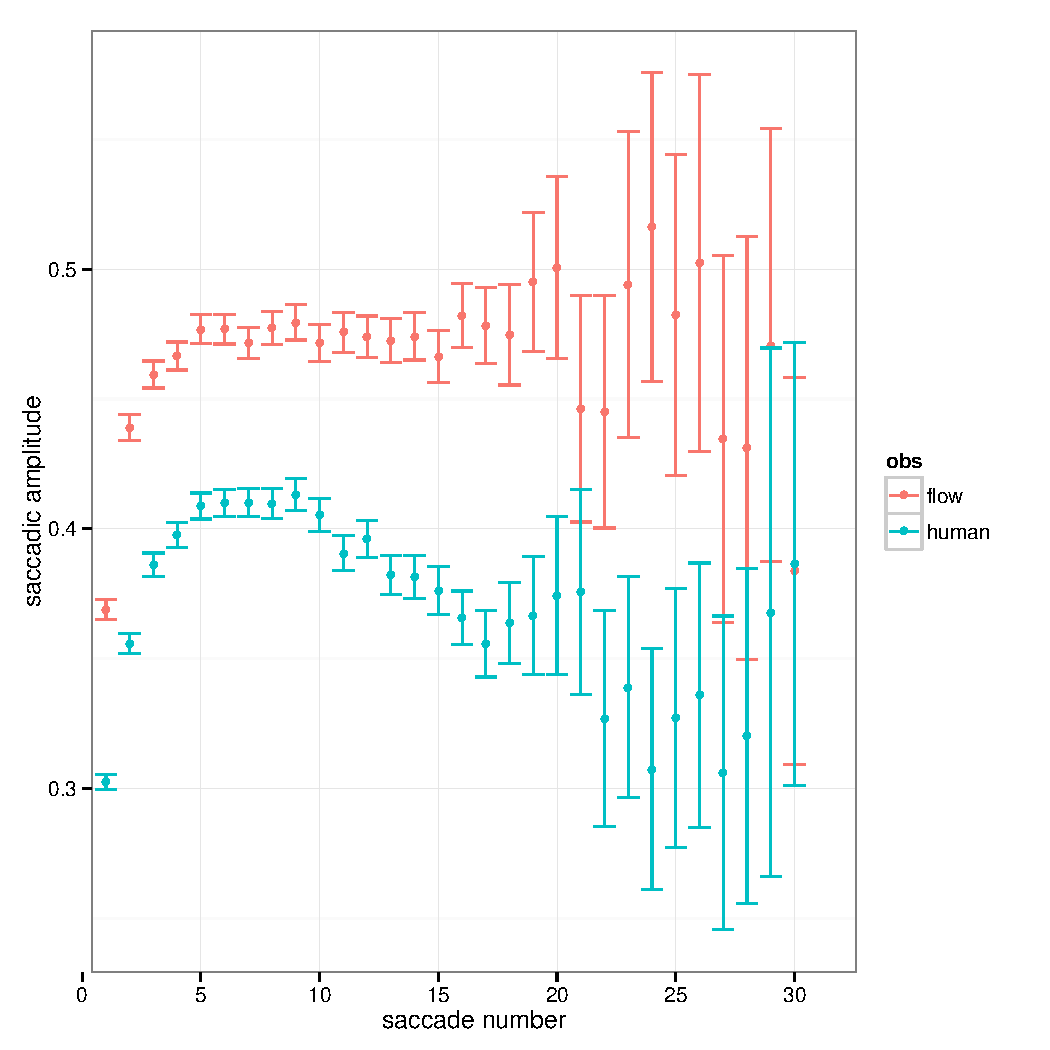
\includegraphics[width=3.8cm]{../scripts/coarse2fine/figs/saccAmpOverTimeFlow}}
\caption[]{\textit{blue}: human, \textit{red}: central bias, \textit{green}: saccadic flow. \textit{top row}: Comparison of $x$ and $y$ fixation positions between human fixations and synthetic points generated from the central bias and flow model. \textit{bottom row}: We can see that the flow model consistently makes saccades with a slightly larger amplitude than human observers. Distances are expressed relative to the width of the image. Best fit line in (d) fitted with loess regression. All distances are given in normalised units in which the width of an image is 2 (see Section \ref{sec:modellingMethods}).}
\label{fig:flowHumanComp}
\end{figure}

\subsection{Discussion}

We have demonstrated different ways biases such as saccadic flow and the central bias can be used in eye movement research. They can be used as a prior on the probability of making saccades to different regions of the image, allowing us to then more clearly visualise the image-dependant behaviour. The likelihood of fixations under the bias models are related to features such as salience, with the interpretation of visual salience as a predictive model of fixation selection being informed by considering how likely a saccade is to be generated by these models of oculomotor bias. Finally, we can also use the bias distributions to generate synthetic data that can be used as control points in ROC analysis, and to explore which aspects of human saccadic dynamics are not captured by the simple flow model. 

\section{Modelling Biases}
\label{sec:biases}

In this section, we (i) update the central bias model of \cite{clarke-tatler2014} to make use of a truncated Gaussian distribution that allows us to take the image boundaries into account. (ii) explore the strength of the leftwards bias in relation to the central bias, and (iii) describe the saccadic flow model. 


%%%%%%%%%%%%%%%%%%%%%%%%%%%%%%%%%%%%%%%%%%%%%%%%%%%%%%%%%%
\subsection{Modelling Methods}
\label{sec:modellingMethods}
%%%%%%%%%%%%%%%%%%%%%%%%%%%%%%%%%%%%%%%%%%%%%%%%%%%%%%%%%%

Here, we give an overview of the methods and data used for the saccadic flow modelling.

\subsubsection{Datasets}

We will use a number of previously published datasets, covering a range of tasks, images, and experimental set-ups. This allows us to produce a model that will generalise well to other datasets. The models will be trained on eight of the ten datasets used in \cite{clarke-tatler2014}. We chose to remove the data from \cite{asher2013} from our training set as the images have an aspect ratio of 5:4, whereas the rest of the data in our training set has an aspect ratio of 4:3. The pedestrian search dataset \citep{ehinger2009} was removed from the training set as previous analysis \citep{clarke-tatler2014} shows that it is biased compared to the other datasets analysed. Both of these datasets are now used as test sets to evaluate how well our models generalise. The initial saccade after image onset ($9.1\%$ of the data) are excluded, giving us a total of 159,226 saccades. An overview of the datasets used is given in Appendix Tables \ref{tab:datasets} and \ref{tab:setuptable}. 


We also add a number of new datasets to the ten used by \cite{clarke-tatler2014}. These will be used to test the model. 

\begin{itemize}

\item \cite{jiang2014} collected data from 16 observers viewing 500 natural scenes containing crowds of people (aspect ratio 4:3).

\item \cite{clarke2009} investigated visual search for a target on a homogeneous textured background (i.e. target in noise). This dataset differs from the previous in that there is no semantic image content in the scene, and the stimuli had a 1:1 aspect ratio.

\item \cite{greene-wolfe2012} released a dataset of observers viewing square greyscale photographs.

\item \cite{borji2015} recently released a very large ($\approx 0.625$million fixations, 2000 images) dataset collected over twenty different stimuli types. Given the size of this dataset, and the wide-screen 16:9 aspect ratio, the evaluations on this dataset are presented separately, and split by stimuli class.

\end{itemize}


\subsubsection{Pre-processing}

As with \cite{clarke-tatler2014}, we have normalised all fixations to the image frame, keeping the aspect ratio constant. i.e., $(x,y)\in (-1.-1)\times(-a,a)$ with typically $a=0.75$. The initial fixations and saccades were not included in the analysis. Saccades with a start or end point falling outside of the image frame were also removed. 

When fitting saccadic flow models, we \textit{mirrored} the set of fixations, by adding in horizontally and vertically reflected copies of the data. This has two advantages. (i) It is an easy way to make the saccadic flow bias symmetric in the horizontal or vertical directions. This is similar to how the central bias was defined \cite{clarke-tatler2014}. (ii) It increases the amount of data available for fitting by a factor of four. This is important as (due to the central bias) there are relatively few saccades that originate from the corners of the images. By equating all corners, we can pool the data and obtain more stable estimates for the underlying distribution. The downside of mirroring saccades in this manner is that our model of saccadic flow will be insensitive to the \textit{leftwards} bias in natural scene viewing \citep{nuthmann-matthias2014}. This will be discussed in Section \ref{sec:LeftRight}. Similarly, as we do not factor in the timecourse of the scanpath, we will not capture \textit{corase-to-fine} dynamics (discussed above in Section \ref{sec:humanComp}).


\subsection{Truncated Central Bias}
\label{sec:truncatedCentral}

First, we will update the central bias from \cite{clarke-tatler2014} and use a truncated normal distribution. This is very straight forward. Re-fitting a multivariante gaussian to the data reduces the deviance in the central bias model by $4.4\%$. Usng a truncated Gaussian gives us an improvement of $12\%$. We can round the truncated Gaussian model to $\mu = (0,0)$, with a covariance matrix of $(0.32, 0; 0, 0.144)$ with no loss of precision. i.e. this is identical to \cite{clarke-tatler2014} except with $\sigma=0.32$ rather than $0.22$

\subsection{Left v Right}
\label{sec:LeftRight}

As mentioned above, the downside of mirroring the saccades in our dataset is that our bias model will be symmetric and will be unable to exhibit the leftwards bias observer in human fixation data. Here, we investigate the size of the leftwards bias. Figure \ref{fig:leftrightDist}) shows that while we do have a leftwards bias in our data, it is apparently a small effect that only last for the first five fixations after scene onset. Furthermore, there is no sign of an asymmetry in the vertical direction.

\begin{figure}
\centering
\subfigure{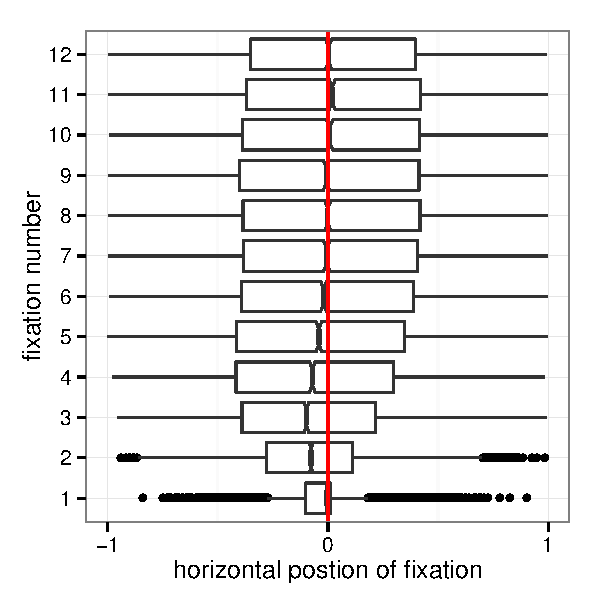
\includegraphics[width=3.8cm]{../scripts/leftVright/graphs/leftrightbias.pdf}}
\subfigure{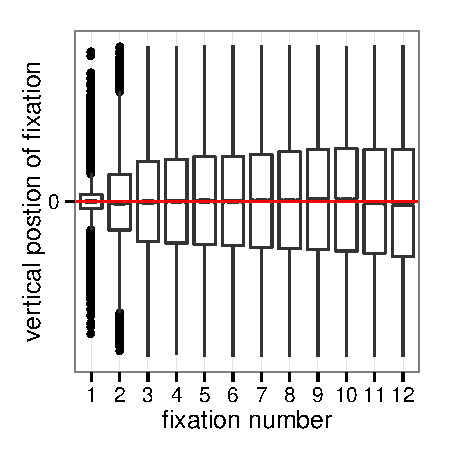
\includegraphics[width=3.8cm]{../scripts/leftVright/graphs/updownbias.pdf}}
\caption{Boxplots showing the distribution of horizontal and vertical fixations by fixation number in the merged training set}
\label{fig:leftrightDist}
\end{figure}

Fitting an ANOVA to predict the $x$-coordinates of the fixations given the fixation number gives adjusted $R^2=0.004$. If we limit our analysis to the first five fixations in each scanpath, this only increases to adjusted $R^2=0.01$. This suggests that by treating everything as symmetrical, we lose little explanatory power, while restricting the number of parameters, or increasing the amount of data available (by mirroring fixations). 

\subsection{Saccadic Flow}
\label{ModellingFlow}

Saccadic flow can be thought of as a generalisation of the central bias., and is illustrated in Figure \ref{fig:empiricalSaccadicFlow}. Instead of computing the distribution of all saccadic endpoints in a dataset, we look at the distribution of saccade endpoints given the start points. I.e.,for a saccade from $(x_0, y_0)$ to $(x_1, y_1)$ we want to model $p(x_1,y_1|x_0, y_0)$.

\subsubsection{Modelling}

To characterise how the distribution of saccadic endpoints varies with the start point, we used a sliding window approach. All saccades that originated from a $n\times n$ window were taken and used to fit a truncated multivariate Gaussian distribution using the \texttt{tmvtnorm} library for \texttt{R}. This window was moved in steps of $s=0.01$ from $[-1,-0.75]$ to $[1-n, a-n]$. Windows containing less than 250 datapoints were discarded. We experimented with varying the window size ($n\in\{0.05,0.1, 0.2\}$). However, as this parameter was found to have a negligible result, we only report the results for $n=0.05$.

Multivariate polynomial regression was then used to fit 4-th order polynomials to each of the parameters. As polynomial regression performs poorly in the presence of outliers, we will also use robust estimation (\texttt{rlm} from the \texttt{MASS} library). This will the model fits being overly influenced by outlier points from the image boundary. 

\subsubsection{Results}

Figure \ref{fig:nParamsOverSpace} shows how the parameters for the truncated multivariate Gaussian distributions vary over horizontal position for a selection of vertical positions. The regression coefficients (given in supplementary materials) allow us to estimate the conditional probability of a saccade to $(x_1, y_1)$ given the starting fixation $(x_0, y_0)$. As the robust estimation methods give a far better fit to the data, we will use this version of the model and discard the polynomial regression version.

\begin{figure*}
\centering
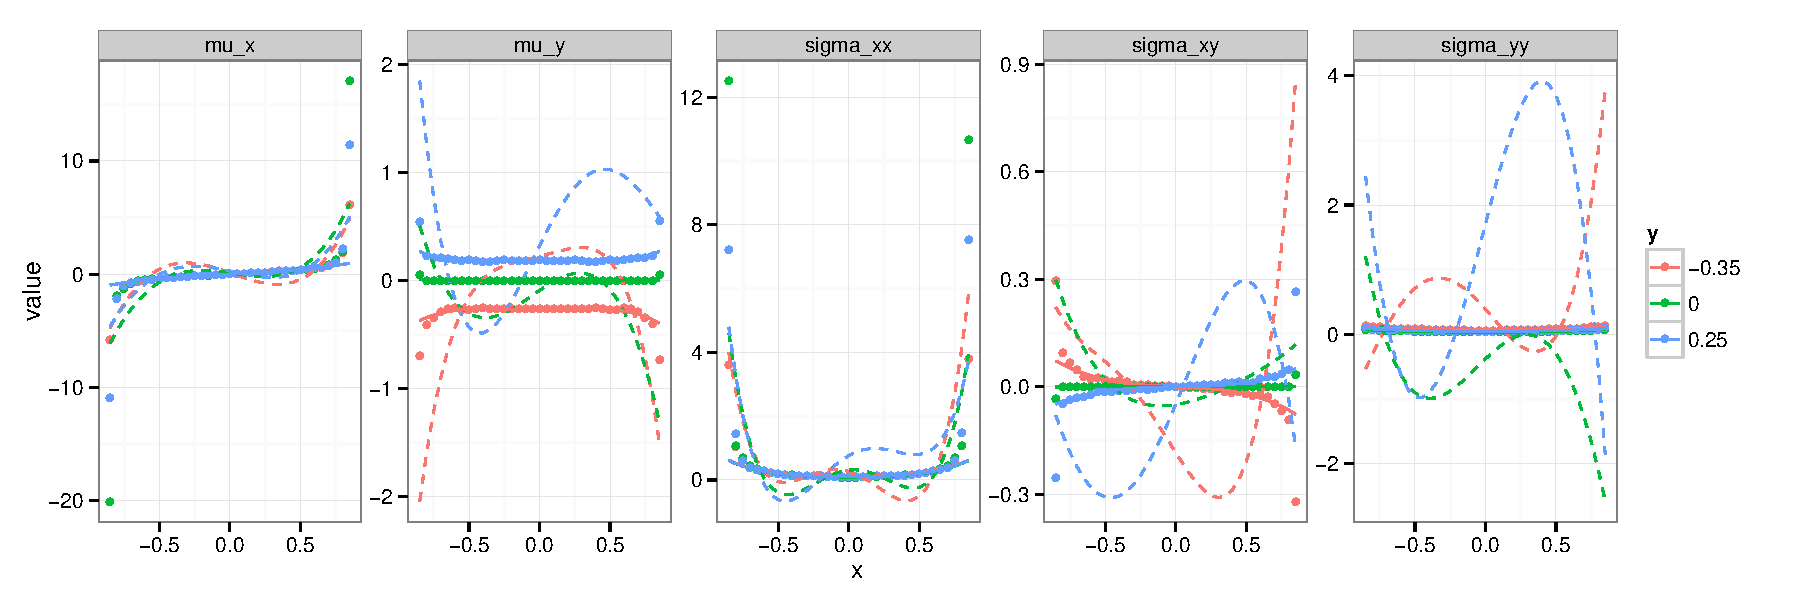
\includegraphics[width=16cm]{../scripts/flow/figs/NparamsChagingOverSpace_ALL_tN}
\caption{How the truncated Gaussian parameters vary with saccadic starting location. Dotted line show polynomial regression fits, solid line shows robust polynomial regression.}
\label{fig:nParamsOverSpace}
\end{figure*}


How well does this model account for the fixations in our datasets? Figures \ref{fig:nFlowDevAll}, \ref{fig:nFlowDevAll2} and \ref{fig:nFlowDevBorji} compared the log-likelihood of the flow model compared to the \cite{clarke-tatler2014} central baseline and a uniform distribution. We can see that in all cases, the log likelihood for the data under the flow model is a lot higher the central baseline and the uniform distribution. It is interesting to note that this holds even for datasets (those involving visual search) in which the central bias is outperformed (terms of log-likelihood) by the uniform distribution: chiefly the data from \cite{clarke2009,asher2013,tatler2007}. 



\begin{figure*}
\centering
 \includegraphics[width=12cm]{../scripts/flow/figs/llh_training.pdf}
\caption{Flow:normal log likelihood results. We can see that re-fitting the central-bias to each specific dataset offers little improvement over using the Clarke-Tatler model, while the flow model offers a substantial improvement.}
\label{fig:nFlowDevAll}
\end{figure*}

\begin{figure*}
\centering
\includegraphics[width=12cm]{../scripts/flow/figs/llh_testing.pdf}
\caption{Doing the same but with some new testing datasets!}
\label{fig:nFlowDevAll2}
\end{figure*}

\begin{figure*}
\centering
 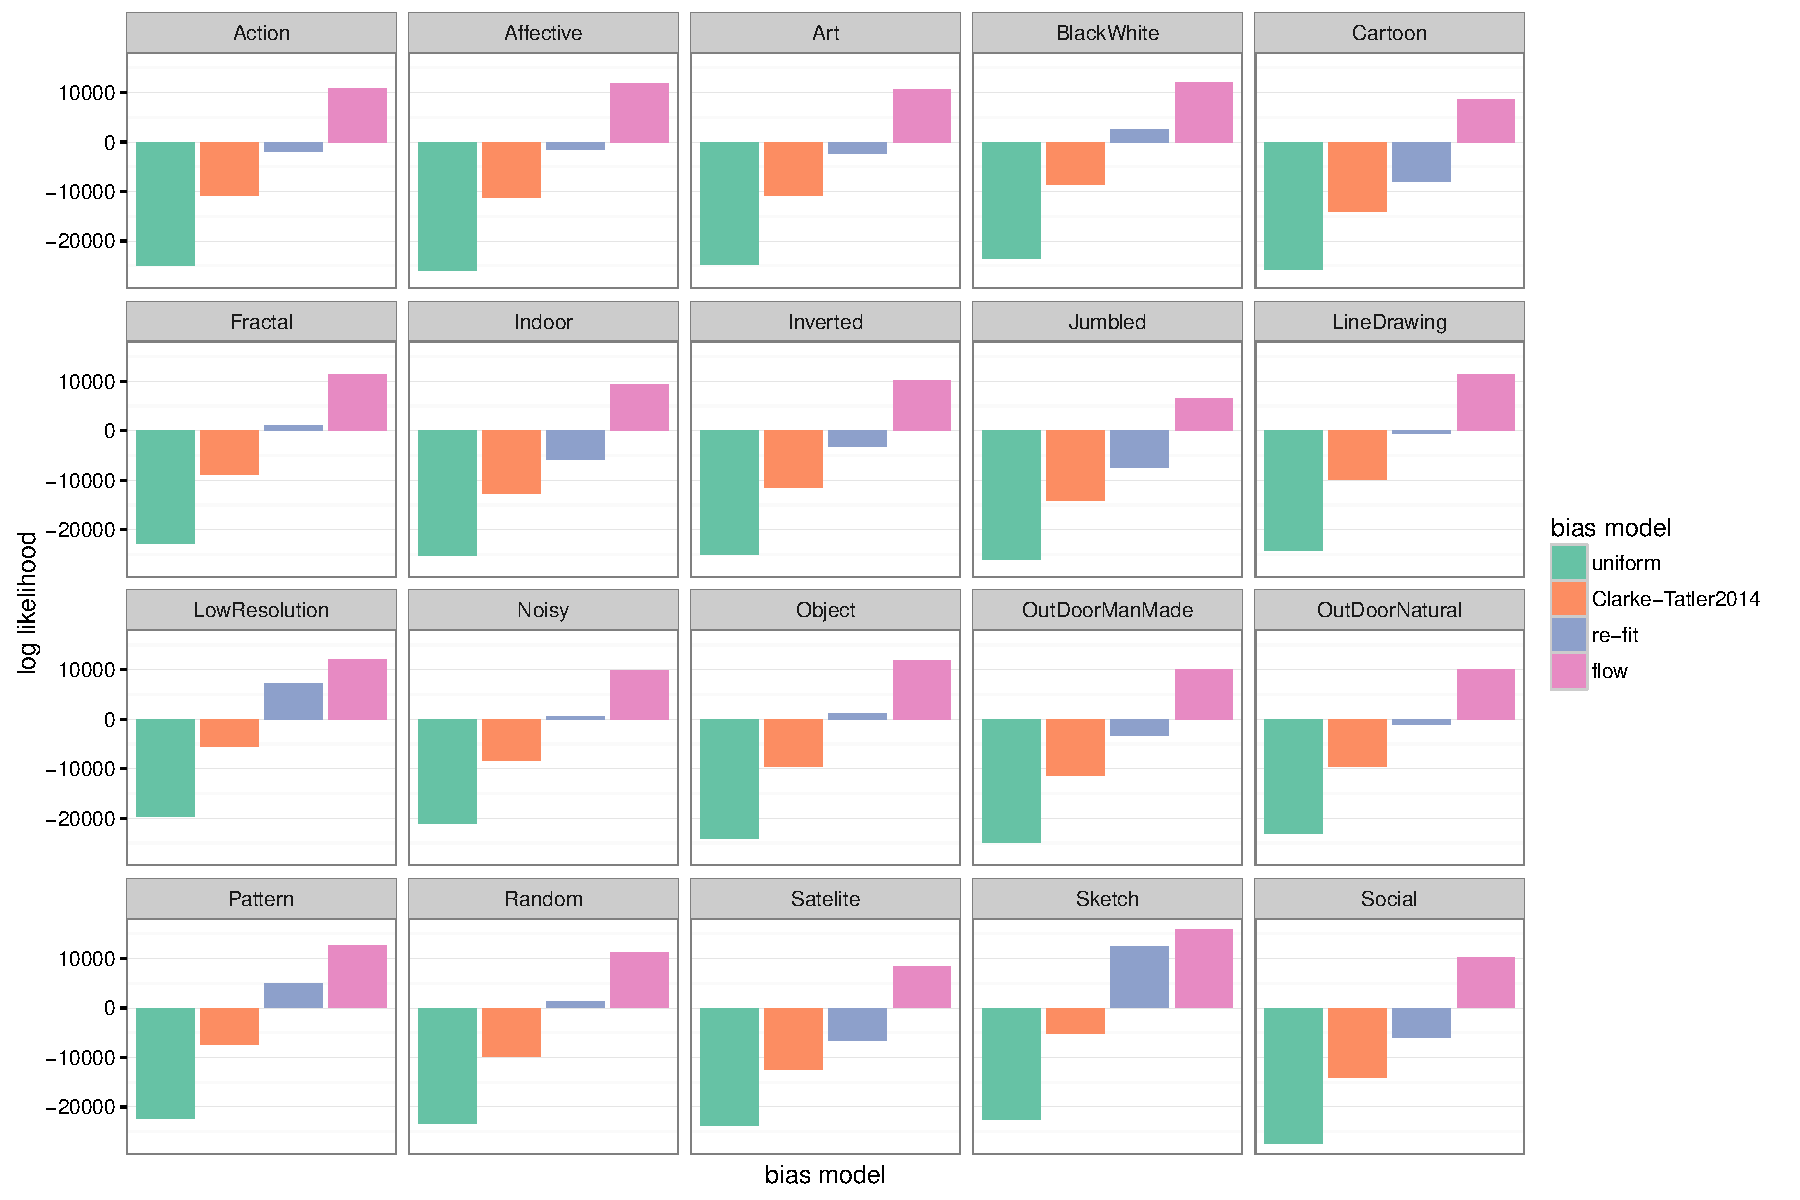
\includegraphics[width=12cm]{../scripts/flow/figs/llh_Borji.pdf}
\caption{Flow:normal deviance results. We can see that re-fitting the central-bias to each specific dataset offers little improvement over using the Clarke-Tatler model, while the flow:normal model decreases the deviance by half.}
\label{fig:nFlowDevBorji}
\end{figure*}

% \begin{figure}
% \centering
%  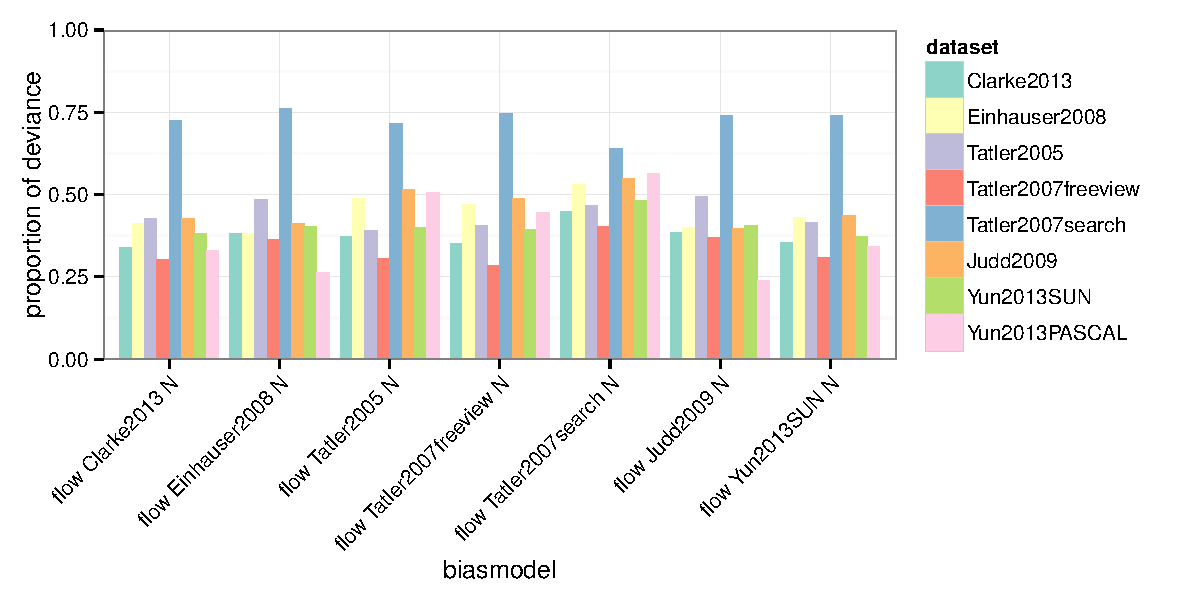
\includegraphics[width=12cm]{../scripts/flow/figs/llh_crossDataset.pdf}
% \caption{Flow:normal deviance results over datasets. In general, we can see that bias models trained on different datasets all explain around the same amount of variance in the datasets.}
% \label{fig:nFlowDevCross}
% \end{figure}

\section{Discussion}
There has been much effort to generate a predictive model of human eye movements \citep{mit-saliency-benchmark,judd2009}. We propose the saccadic flow model as a robust prior for the image-content independent saccadic behaviour that is evident when people look at pictures \citep{tatler-vincent2009}. There are two ways in which models of eye movements may benfit from including such information. First, models may include saccadic flow in their calculation of spatial prediction. Understanding where someone is currently fixating in an image appears to dramatically influence where they will go next, meaning that as saccadic flow can be parametrically estimated from any point on an image, it may be that this can be used to weight models of low-level (i.e. visual conspicuity) and high-level (i.e. semantic interest) features. Thus, whether someone fixates one of two equally conspicuous, equally interesting objects may be simply determined by the way that the eyes \textit{tend} to move. 

The second potential utility of saccadic flow is to generate realistic control fixations with which to compare observed fixation data. In this way, saccadic flow can be thought of as a partner to the \cite{clarke-tatler2014} central bias, and we expect that in some cases, the simpler central bias will be more appropriate. However we have demonstrated that while the flow model requires more parameters (we use 16 coefficients to track how each of the five truncated Gaussian parameters vary as as a function of $(x,y)$), it generalises well from one dataset to another and is a far better baseline for modelling a scan-path than the central bias.

There are two main limitations to our modelling work. Firstly, by using a truncated Gaussian we are unable to capture the skewed nature of the distribution of saccades originating from the corners (see Figure \ref{fig:empiricalSaccadicFlow}). We experimented with fitting a skew-normal distribution using the \texttt{sn} package for \texttt{R}, but met with limited success due to having to deal with the image boundaries. We expect this is one of the main reasons why our saccadic flow model generates saccades with on average greater amplitudes than those seen in empirical distributions. The second simplification is that by not taking the leftwards or coarse-to-fine biases into account, we are limiting the degree to which we can model the dynamics of human scan-paths.

\subsection{Conclusions}
Behavioural biases in eye movement are prevelant during scene viewing. Our saccadic flow model allows calculation of saccade likelihood across an image based on empirical data of how the eye tends to move in many different scene viewing conditions, with flow provides a strong fit to a wide number of datasets. There are a number of ways that flow can be developed, and we propose that gaining a better understanding of the saccadic biases underlying fixation behaviour can only be a positive for our search to understand why people look where they look.

%\section{Discussion}


%What isn't captured by our flow model? There will be some stuff in \cite{macinnes2014}

%\subsection{Scenes and natural viewing behaviour}
%That observers organise their viewing behaviour on computer screens around the reference frames provided by the bounds of scenes (see also \cite{stainer2013}) causes problems for relating findings of eye guidance in scenes to eye guidance in natural behaviour, as the bounds of such reference frames are unclear in the real world. While it has been suggested that we tend to fixate near to the centre of our `straight ahead' head position [FOULSHAM WALKING, CRISTINO AND BADDELEY?], there are no discrete edges as are typical in computer based scene viewing paradigms. If fixation locations are constrained by the bounds of the scene, this highlights the care we must take about the generalisations we make from findings in the lab to the real world (see [kingstonepaper 2010]). 


\section*{Acknowledgements}

And mention grants. 

\section*{Author Contribution}

All authors co-wrote the paper. The saccadic flow model was developed by ADFC. The gaze landscapes and saliency analysis were done by MJS.

\appendix
\section{Dataset Details}

Here are all the details on the datasets used in this paper. (Table \ref{tab:datasets} and \ref{tab:setuptable}).


\begin{table*}
\centering
\small
\begin{tabular}{l|llll}
 						& Observers & Images &  Task & Display duration\\
\hline
\cite{clarke2013}     	& 24   	& 100   & object naming & 5000 ms\\
\cite{yun2013} - SUN    & 8     & 104   & image description & 5000 ms\\
\cite{tatler2005}     	& 14    & 48    & memory 			& variable\\
\cite{einhauser2008} 	& 8		& 93    & object naming 	& 3000 ms \\
\cite{tatler2007} - free & 22   & 120   & free viewing      & 5000 ms\\
\cite{judd2009}         & 15 	& 1003  & free viewing 		& 3000 ms\\
\cite{yun2013} - PASCAL & 3 	& 1000  & free viewing 		& 3000 ms\\
\cite{tatler2007} - search & 30 & 120	& visual search 	& 5000 ms\\
\hline
\cite{clarke2009} 		& 7		& 360	& visual search 	& variable\\
\cite{ehinger2009}     	& 14 	& 912 	& visual search 	& variable\\
\cite{asher2013}    	& 25    & 120   & visual search		& variable\\
\cite{jiang2014}  		& 16 	& 500 	& free viewing  	& 5000 ms \\
\cite{borji2015}  		& 120	& 4000  & free viewing		& 5000 ms\\
\end{tabular}

\caption{Summary of the 13 datasets used throughout this study. The top eight datasets were used to train the model, while the bottom five were only used for evaluation.}
\label{tab:datasets}
\end{table*}

\begin{table*}
\begin{center}
\small
\begin{tabular}{l|llllll}
 & Eye tracker & \vtop{\hbox{\strut Viewing}\hbox{\strut distance}}
 & \vtop{\hbox{\strut Screen}\hbox{\strut size}}
 & \vtop{\hbox{\strut Image}\hbox{\strut size}}
 & \vtop{\hbox{\strut Viewing}\hbox{\strut angle}}
 & \vtop{\hbox{\strut Chin /}\hbox{\strut head rest}}\\
\hline
\cite{tatler2005} 			& EyeLink I 	& 60 cm 	& 17" 	& $800 \times 600$ 	& $30 \times 22^{\circ}$ 	& no\\
\cite{tatler2007} - free 	& EyeLink II 	& 60 cm 	& 21" 	& $1600 \times 1200 $	& $40 \times 30^{\circ}$ 	& no \\
\cite{tatler2007} - search 	& EyeLink II 	& 60 cm 	& 21" 	& $1600 \times 1200$ 	& $40 \times 30^{\circ}$ 	& no\\
\cite{einhauser2008} 		& EyeLink 1000 	& 80 cm 	& 20" 	& $1024 \times 768$ 	& $29 \times 22^{\circ}$ 	& yes\\
\cite{judd2009} 			& ? 			& 2 feet 	& 19" 	& $1024 \times 768*$ 	& ? 				& yes\\
\cite{clarke2013} 			& EyeLink II 	& 50 cm 	& 21" 	& $800 \times 600$ 	& $31 \times 25^{\circ}$ 	& no\\
\cite{yun2013} - PASCAL 	& EyeLink 1000	& ? 		& ? 	& ? 			& ? 				& ?\\
\cite{yun2013} - SUN 		& EyeLink 1000 	& ? 		& ? 	& ? 			& ? 				& ?\\
\hline
\cite{clarke2009} 			& Tobii x50 	&87 cm			& 20"		& $1024\times 1024$	&	$16.7\times16.7^{\circ}$ & yes \\
\cite{ehinger2009} 			& ISCAN RK-464 	& 75 cm 	& 21" 	& $800 \times 600$ 	& $23.5 \times 17.7^{\circ}$& yes\\
\cite{asher2013} 			& EyeLink 1000 	& 55 cm 	& ? 	& $1024 \times 1280$& $37.6 \times 30.5^{\circ}$& yes\\
\cite{jiang2014}  			& Eyelink 1000 	& 57 cm		& 22"	& $1024 \times 768$ & $38.8 \times 29.1^{\circ}$& ?\\
\cite{borji2015} 			& Eyelink 1000	& 106 cm	& 42" 	& $1920\times1080 $	&$45.5\times31^{\circ}$& yes \\
\end{tabular}
\end{center}

\caption{Details of the experimental setups in each of the 10 datasets analysed in the present study. We provide only information reported in the original articles. Question marks indicate information not reported in the original article. *For the Judd et al dataset images varied in pixel dimensions but the majority were at 1024 x 768.}
\label{tab:setuptable}
\end{table*}

\bibliographystyle{plainnat}
\small
\bibliography{literature.bib}
\end{document}